%****************************************************************%
% FILE: architettura.tex                                         %
%****************************************************************%
\documentclass[./main.tex]{subfiles}

\begin{document}
 
Lo sviluppo di una grande applicazione necessita di avere un'architettura base nella quale viene definito ogni singolo componente e la relazione con gli altri, sia per separare logicamente il lavoro che per assegnarlo a diversi membri del team in modo che possano procedere allo sviluppo nello stesso momento. 

% PARAGRAPH: descrizione schema 
%\paragraph{Schema.}
Lo schema presente in \autoref{fig:arch} mostra i diversi elementi che compongono l'infrastruttura di \textit{Ismar Data}. La più grande divisione avviene tra \textbf{front-end} e \textbf{back-end}. Il primo rappresenta la vera e propria applicazione che l'utente andrà ad utilizzare, quindi consiste nello sviluppo della grafica e delle richieste al back-end per ottenere i dati da visualizzare. Il back-end invece rappresenta le fondamenta. Si occupa del reperimento dei dati, della loro elaborazione, del salvataggio all'interno di un database e della creazione delle \textbf{API}\footnote{infra, pp. 61-63.} (\textit{Application Programming Interface}) necessarie al reperimento di essi. Nei successivi paragrafi saranno trattati i singoli blocchi presenti nello schema, dando un'idea semplice del perché sono stati inseriti nel disegno.\par

% img schema architettura %
\begin{figure}[!ht]
\noindent\begin{minipage}{\textwidth}
\vspace{1cm}
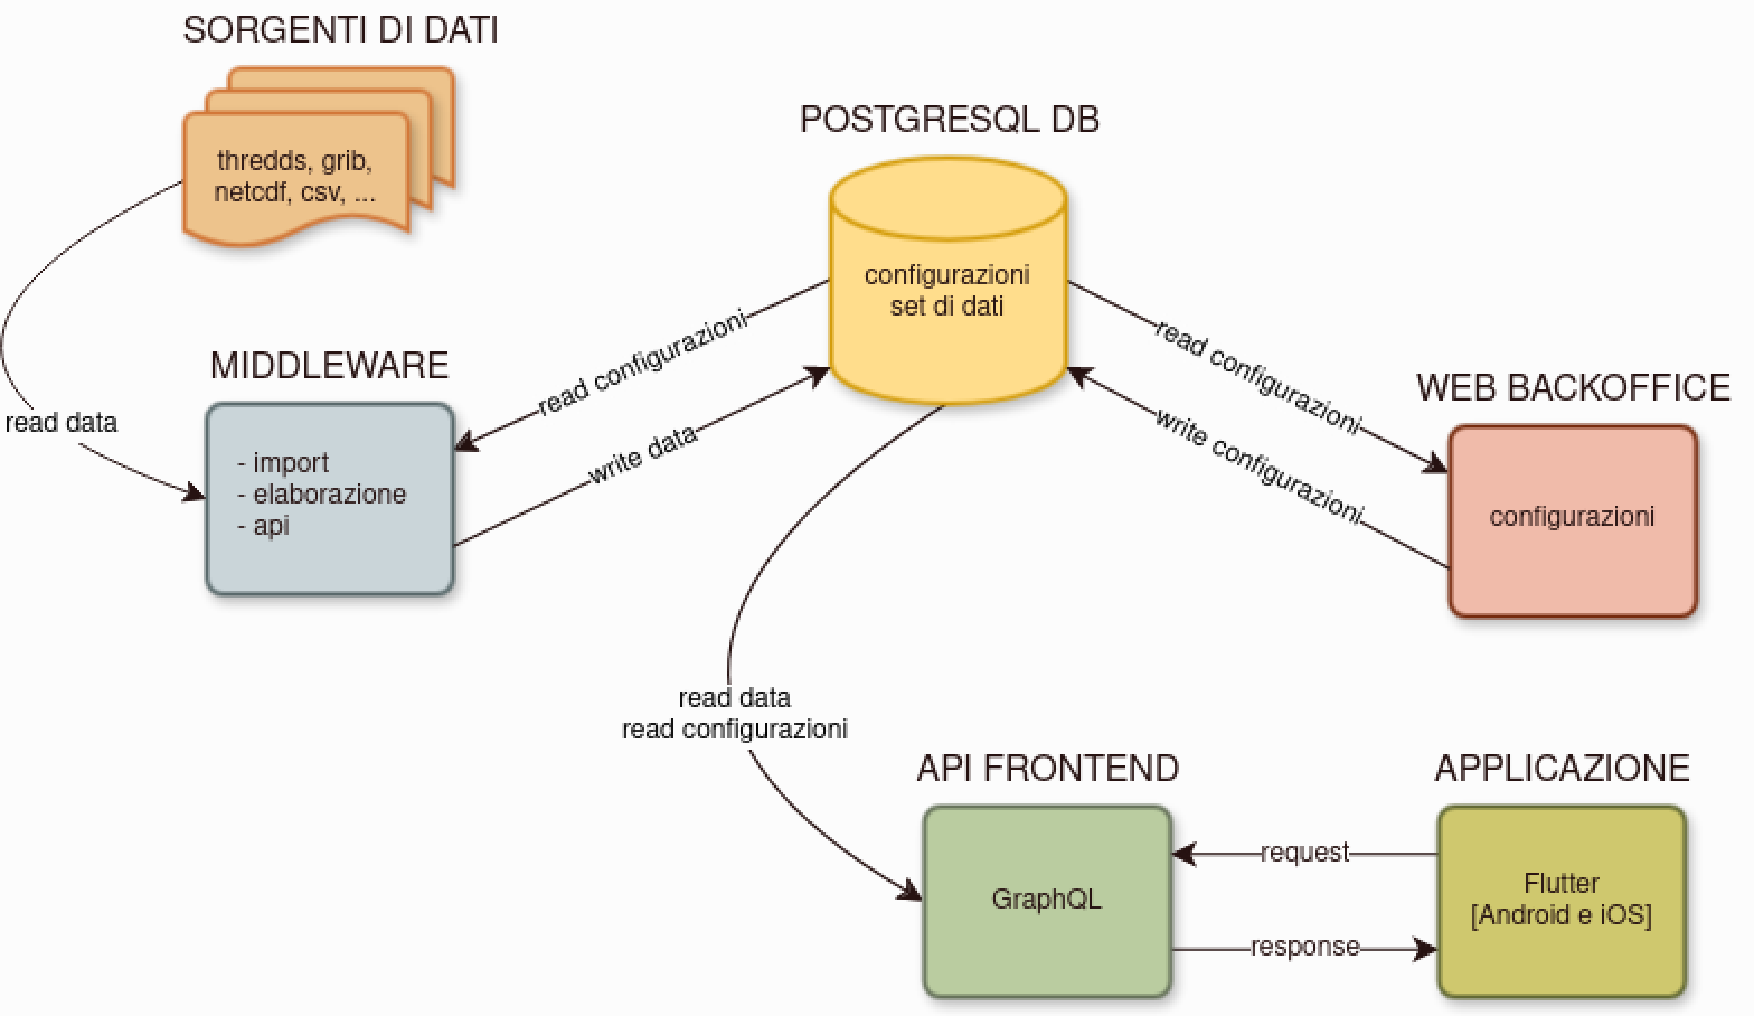
\includegraphics[width=\textwidth]{images/architettura.pdf}
\captionsetup{font=small, hypcap=false}
\captionof{figure}{Schema architettura. (Diagramma creato utilizzando drawio\footcite[\url{https://www.drawio.com/}]{website-drawio}).}
\label{fig:arch}
\end{minipage}
\vspace{0.25cm}
\end{figure}
% PARAGRAPH: database 
%\paragraph{PostgreSQL}
L'entità centrale è il database relazionale \textbf{postgreSQL}\footcite[\url{https://www.postgresql.org/}]{website-postgres}. Al suo interno sono conservati tutti i dati necessari al funzionamento dell'applicazione. È stato scelto un database di questo tipo in quanto funziona su tutti i sistemi operativi maggiormente utilizzati, è \textit{open-source}, è sicuro e interagisce bene con le altri componenti. Inoltre, essendo relazionale, consente di avere uno schema ben strutturato con entità (tabelle) e relazioni tra esse, utile per i dati \textit{statici}. Con questo termine si intendono i dati riguardanti le infrastrutture vere e proprie (vedi esempio di piattaforma in \autoref{fig:aaot})  che si occupano della raccolta dei dati tramite i sensori. Le informazioni riguardanti i sensori raramente evolvono nel tempo e hanno dati molto simili tra loro (ad esempio il tipo di sensore utilizzato viene spesso ripetuto, o l'ente proprietario), dunque il salvataggio in un database relazionale è la scelta più adatta. Per quanto riguarda invece i dati dinamici, la situazione si complica. Inizialmente era stato previsto un ulteriore database, non relazionale perché sono dati diversi tra loro,  per il salvataggio di essi. Si sarebbe dovuto interfacciare con il \textit{middleware} e le \textit{API front-end}. Il problema è che questi dati, come accennato nell'introduzione del documento, non sempre sono accessibili. Quindi la soluzione del secondo database è stata momentaneamente archiviata. I pochi dati disponibili, dopo un'attenta elaborazione, vengono salvati nel database principale PostgreSQL. Operazione possibile grazie a diversi meccanismi per l'aggiornamento delle nuove informazioni e l'eliminazione dei dati meno recenti, mantenendo uno storico, come da richiesta del cliente, di 10 giorni indietro dalla data odierna e di 5 giorni avanti per le eventuali previsioni.\par

% img piattaforma acqua alta %
\begin{figure}[!ht]
\noindent\begin{minipage}{0.5\textwidth}
\vspace{1cm}
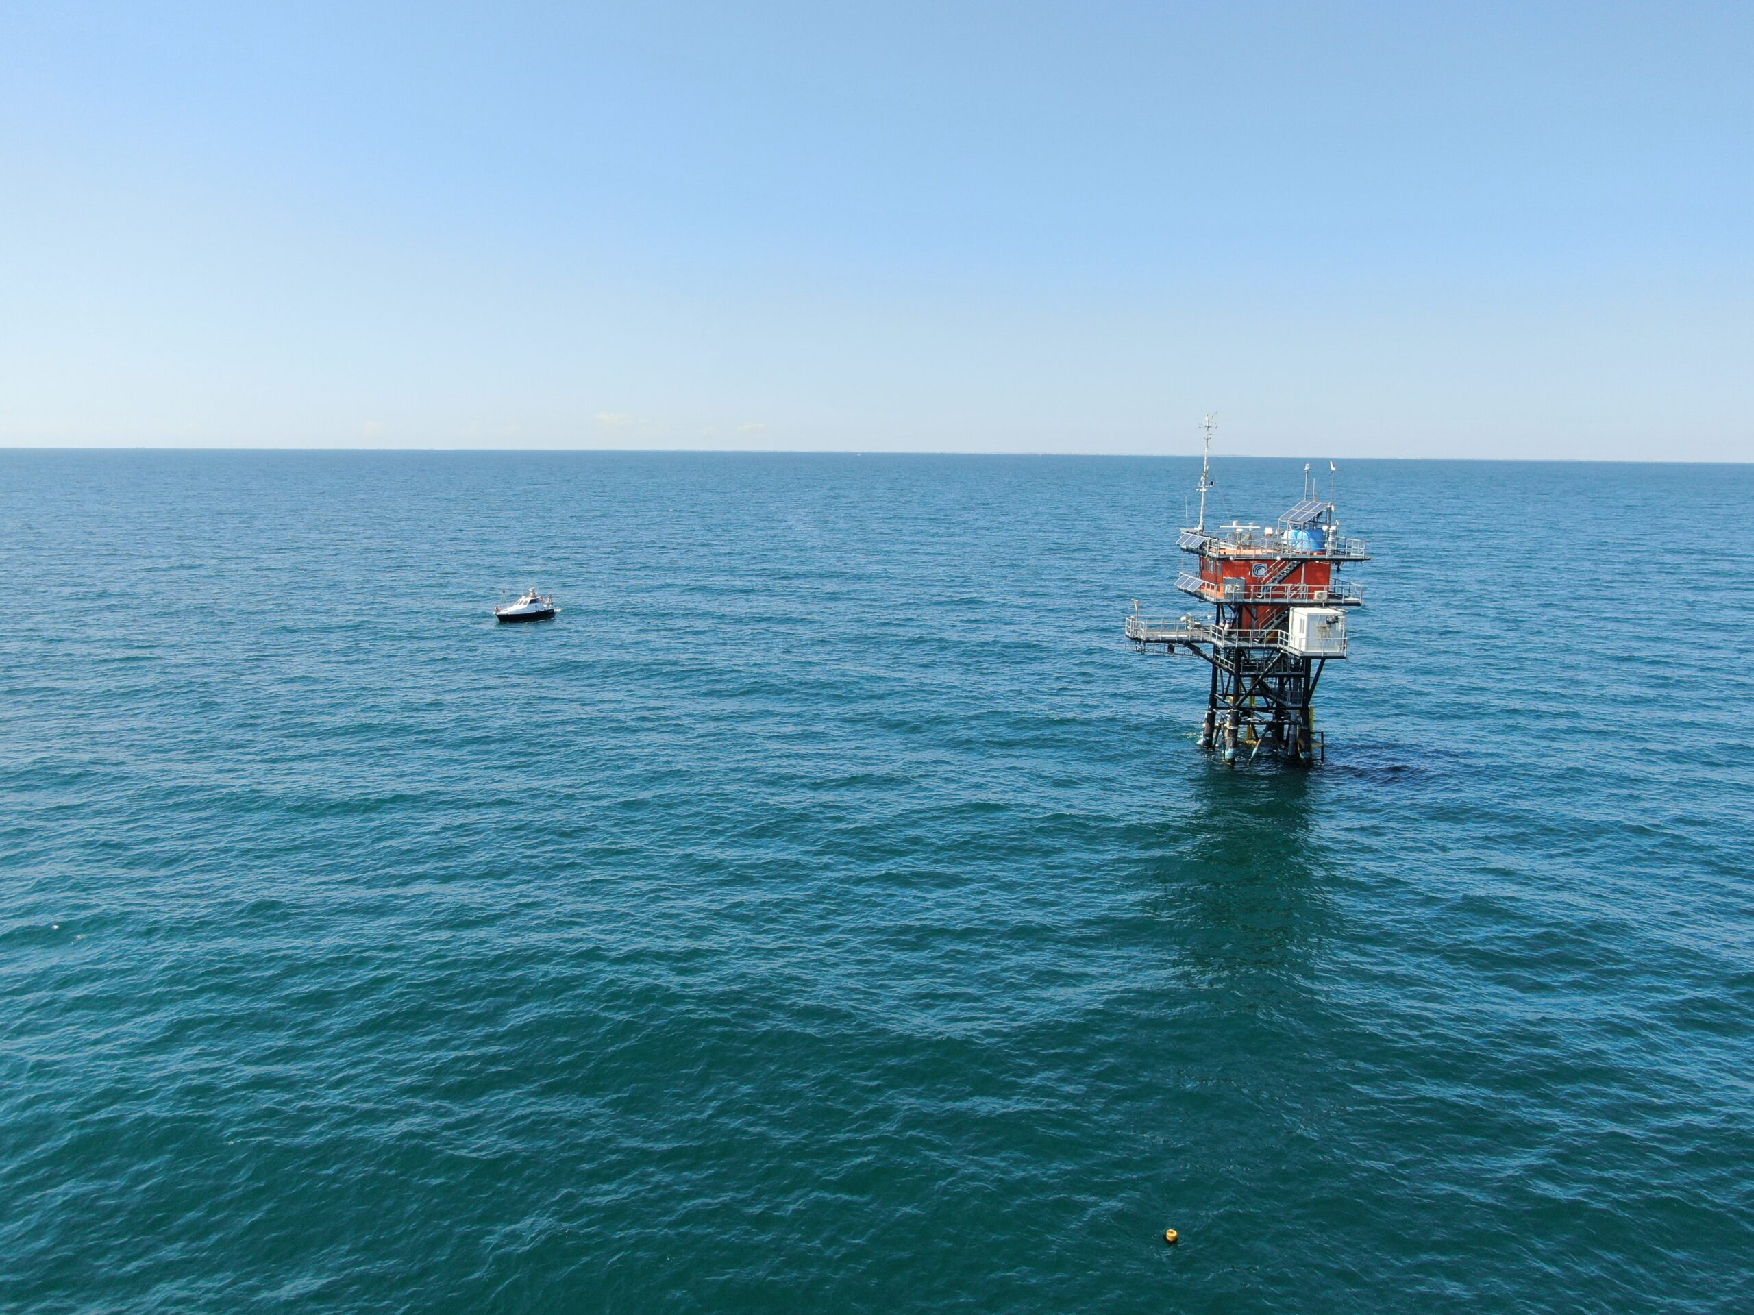
\includegraphics[width=\textwidth]{images/aaot.pdf}
\captionsetup{font=small, hypcap=false}
\captionof{figure}{Piattaforma Oceanografica Acqua Alta\protect\footcite[Fonte: ][\url{https://www.ismar.cnr.it/wp-content/uploads/2023/06/PTF-2018-07-scaled.pdf}]{website-ismar-cnr}.}
\label{fig:aaot}
\end{minipage}
\hspace{0.05\textwidth}
\begin{minipage}{0.4\textwidth}
\begin{small}
La Piattaforma Oceanografica Acqua Alta è situata a circa 8 miglia al largo del litorale di Venezia, in uno specchio di mare avente una profondità di circa 16 m (GPS 45.3142467 N, 12.5082483 E)\footcite[\url{https://www.ismar.cnr.it/infrastrutture/infrastrutture-oceanografiche/piattaforma-acqua-alta/}]{website-ismar-cnr}.
\end{small}
\end{minipage}
\vspace{0.25cm}
\end{figure}

% PARAGRAPH: web backoffice   
%\paragraph{Web Backoffice.}
Il Web Backoffice è un semplice applicativo web, implementato tramite \textbf{Django}\footcite[\url{https://www.djangoproject.com/}]{website-djangoproject},  per la gestione e configurazione dei dati statici. Una schermata è mostrata in \autoref{fig:bo}.  Django, tra le sue funzionalità, implementa anche un'interfaccia di amministrazione. Essa esiste come strumento per ispezionare e gestire i dati del database, non va considerata come un'interfaccia pubblica dei dati\footcite[102-103]{the-django-book}.\par

% img web backoffice %
\begin{figure}[!ht]
\noindent\begin{minipage}{0.5\textwidth}
\vspace{1cm}
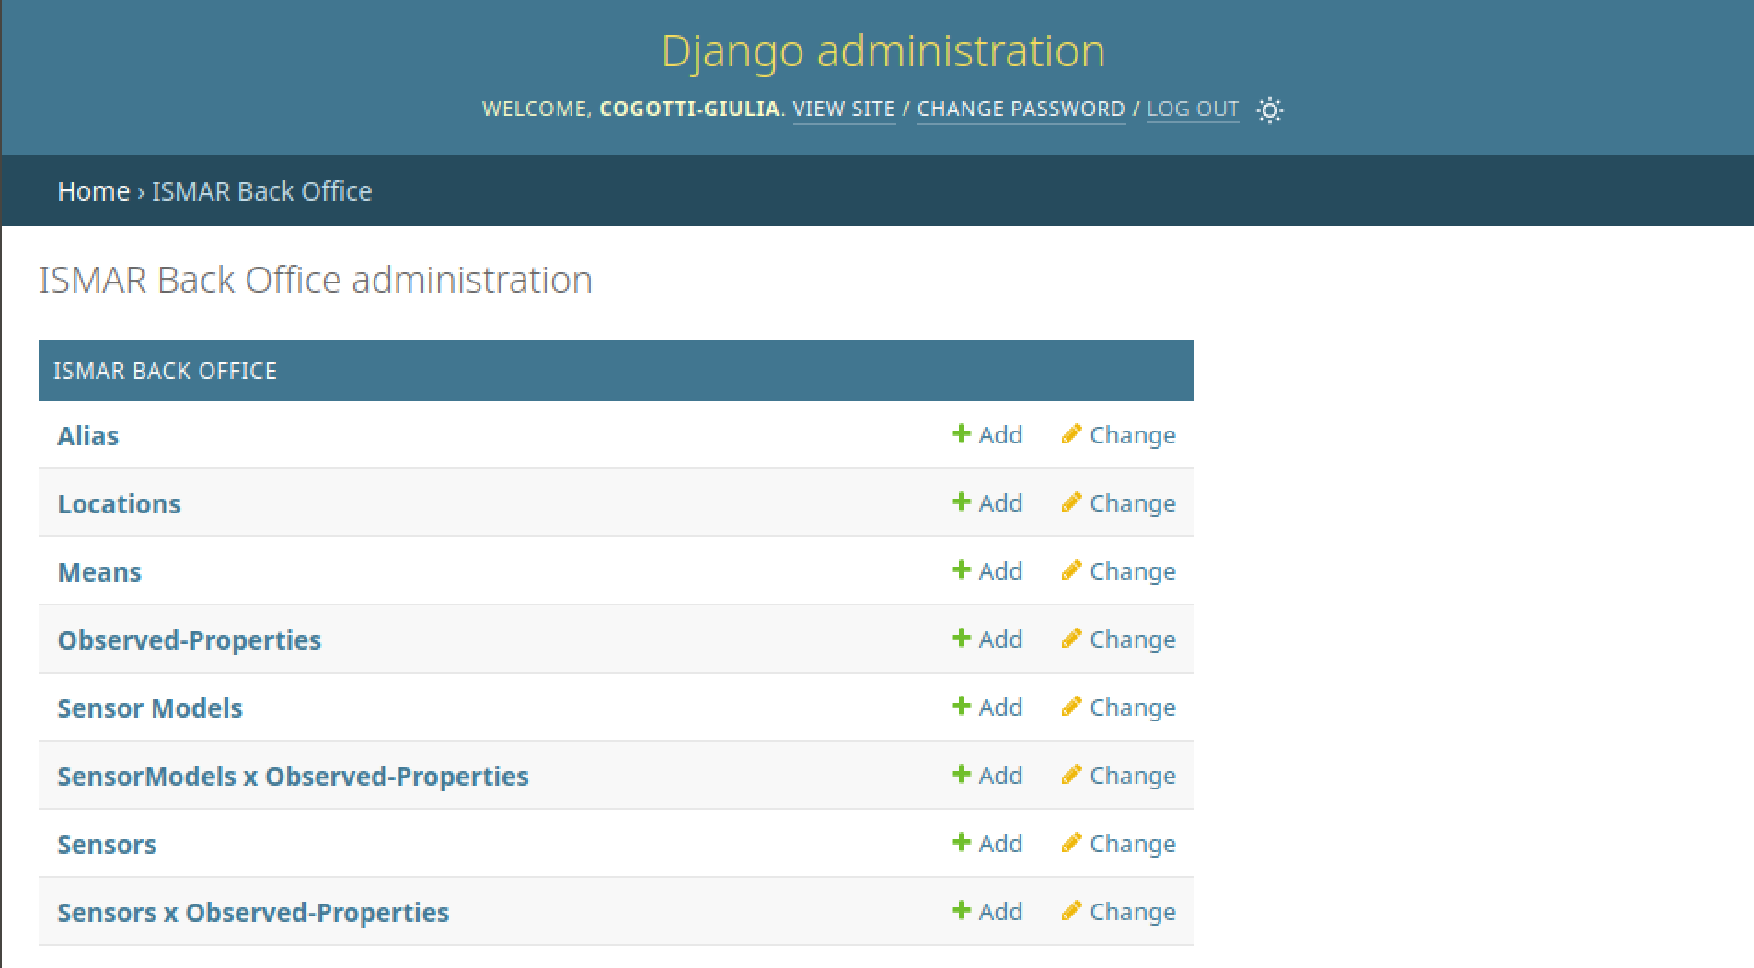
\includegraphics[width=\textwidth]{images/sample_backoffice.pdf}
\captionsetup{font=small, hypcap=false}
\captionof{figure}{Sito amministrazione backoffice\protect\footnote{Fonte: screenshot dall'autrice.}.}
\label{fig:bo}
\end{minipage}
\hspace{0.05\textwidth}
\begin{minipage}{0.4\textwidth}
\begin{small}
Esempio di interfaccia del sito di amministrazione, richiede credenziali di accesso e rispecchia i modelli del database.
\end{small}
\end{minipage}
\vspace{0.25cm}
\end{figure}

% PARAGRAPH: sorgenti di dati
%\paragraph{Sorgenti di dati.}
Le sorgenti sono l'insieme di dati provenienti dalle varie fonti con tipi e modalità differenti. I dati rappresentano tutte le misurazioni effettuate dai sensori posti nelle stazioni e radar analizzati, dunque sono variabili nel tempo.\par

% PARAGRAPH: middleware
%\paragraph{Middleware.}
Il middleware è la componente che si occupa di prelevare i dati "grezzi", filtrarli ed eventualmente salvarli sul database. Questo passaggio è indispensabile per diverse ragioni. Innanzitutto le sorgenti raccolgono una mole di dati superiore a quella che effettivamente serve al funzionamento dell'applicazione, dunque prendere solo il necessario rende il progetto più leggero. Risulta opportuno ricordare che l'applicazione sarà utilizzata da un utente che si aspetta un tempo di risposta ragionevole, compreso tra i 0.1 e 10 secondi\footcite[268-276]{Miller68-0}. L'accesso ad alcune categorie di dati richiede un tempo non indifferente, decisamente superiore al limite, quindi il presalvataggio (effettuato durante l'orario di aggiornamento delle sorgenti, solitamente orario notturno) consente di evitare questo tipo di problematiche.\par

% PARAGRAPH: API front end  
%\paragraph{API front-end.}
Il passaggio dei dati al lato grafico dell'applicazione avviene tramite API front-end che leggono i dati e le configurazioni presenti nel database. Come linguaggio di interrogazione al database si è scelto di utilizzare GraphQL\footcite[\url{https://graphql.org/}]{website-graphql}.\par

% PARAGRAPH: app mobile 
%\paragraph{Applicazione.}
L'unica parte riguardante il front-end si focalizza sull'applicazione mobile. Essa sarà sviluppata utilizzando il framework Flutter\footcite[\url{https://flutter.dev/}]{website-flutter} in quanto risulta semplice e veloce da utilizzare. Una caratteristica fondamentale di Flutter è che consente di scrivere codice multi-piattaforma (nel caso specifico, Android e iOS) a partire da un codice base comune. Questo elimina i problemi derivanti dal dover scrivere un'applicazione nativa per il sistema scelto. Il front-end sarà sviluppato da un team esterno, dunque non sarà analizzato nel presente documento.\par

\end{document}
